\documentclass[11pt]{report}
\usepackage{styles/projectreport}
\usepackage{amsmath,amssymb,amsfonts, amsthm}
\usepackage{bbm,bm} 
\usepackage{listings}

\newtheorem{theorem}{Theorem}
\newtheorem{example}{Example}
\newtheorem{remark}{Remark}
\newtheorem{lemma}[theorem]{Lemma}
\newtheorem{assumption}{Assumption}
\newtheorem{corollary}[theorem]{Corollary}
\newtheorem{definition}[theorem]{Definition}

\usepackage{cleveref}

\addbibresource{report/references.bib}

\begin{document}

\setlength{\abovedisplayskip}{3pt} % Set upper buffer space when using align
\setlength{\belowdisplayskip}{3pt} % Set lower buffer space when using align

\newcommand{\N}{\mathbb{N}}
\newcommand{\Z}{\mathbb{Z}}
\newcommand{\R}{\mathbb{R}}
\newcommand{\E}{\mathbb{E}}
\newcommand{\Prob}{\mathbb{P}}
\newcommand{\Ex}{\mathbb{E}}
\newcommand{\I}{\mathbb{I}}
\newcommand{\mean}{\mu}
\newcommand{\naturals}{\mathbb{N}}
\newcommand{\suchthat}{\,\text{\textit{st.}}}

\newcommand{\one}{\mathbbm{1}}
\newcommand{\actionValueEstimate}{$\mathcal{E}$}
\newcommand{\epsilonFunction}{$\varepsilon(t)$}
\newcommand{\gap}[1]{\Delta_{#1}}

\newcommand{\numArms}{K}
\newcommand{\armsList}{A}
\newcommand{\timeHorizon}{T}
\newcommand{\armDistribution}[1]{\mathrm{P}_{#1}}
\newcommand{\maxArmDistribution}{\armDistribution{\star}}
\newcommand{\armPopulationMean}[1]{\mean_{#1}}
\newcommand{\armPopulationMeanSpecific}[2]{\mean_{#1}(#2)}
\newcommand{\maxArmIndices}{\mathrm{J}_{\star}}
\newcommand{\maxPopulationMean}{\armPopulationMean{\star}}
\newcommand{\armDistributionVect}{\mathrm{P}}
\newcommand{\banditSpace}{\xi}
\newcommand{\aBandit}{\mean}

\newcommand{\bandit}{\nu}
\newcommand{\aDifBandit}{\bar{\bandit}}
\newcommand{\vectorBanditMeans}{\hat{\bandit}}

\newcommand{\totalFunction}[2]{\mathbb{T}_{#1}(#2)}
\newcommand{\ucb}[3]{\mathrm{UCB}_{#1}^{#3}(#2)}
\newcommand{\ucbPolicy}{\policy_{\mathrm{UCB}}}

\newcommand{\empiricalMeanReward}[2]{\hat{\mean}_{#1}(#2)}
\newcommand{\maxMeanArm}{\mathrm{M}}
\newcommand{\maxTrueArms}{\mathrm{N}}
\newcommand{\relativeEntropy}[2]{D(#1, #2)}

\newcommand{\failureProb}{\delta}
\newcommand{\stoppingTime}{\mathcal{T}}
\newcommand{\selectionRule}{\mathcal{S}}
\newcommand{\method}{\mathcal{M}}

\newcommand{\action}[1]{A_{#1}}

\newcommand{\reward}[2]{
   \ifthenelse{\isempty{#2}}{
   Y_{#1}(\action{#1})}{
   Y_{#1}(#2)}}

\newcommand{\policy}{\varphi}

\newcommand{\cumulativeRegret}[2]{\mathcal{R}_{#1}(#2)}
\newcommand{\simpleRegret}[2]{\mathcal{R}_{#1}(#2)}

\newcommand{\commented}[1]{}

\newcommand{\seperator}[0]{\centerline{\rule{0.5\textwidth}{0.4pt}}}

\SetKwFunction{policyTAS}{policyTAS}
\SetKwProg{Fn}{Function}{:}{}


\newcommand{\defineVagueZedTee}[1]{\inf\limits_{\aDifBandit \in \banditSpace_{alt}(\vectorBanditMeans(#1))}
\sum_{i=1}^k \totalFunction{i}{#1} \relativeEntropy{\bandit_{i}}{\bandit_{i}^{'}}}

\newcommand{\defineZedTee}[1]{\frac{1}{2}\inf\limits_{\aDifBandit \in \banditSpace_{alt}(\vectorBanditMeans(#1))}
\sum_{i=1}^k \totalFunction{i}{#1} \left( \vectorBanditMeans_i - \aDifBandit_i \right)^2}

\newcommand{\failureProbabilityFunction}{f}

\newcommand{\minsub}{\min_{i \not\in \maxArmIndices}}

\newcommand{\bigO}[1]{\mathcal{O}(#1)}

\newcommand{\sumindgreater}{\sum_{i=1}^{K} \one_{\{\Delta_i \geq \epsilon\}}}

\newcommand{\sumindless}{\sum_{i=1}^{K} \one_{\{\Delta_i \leq \epsilon\}}}

\newcommand{\placeholder}[1]{
\begin{figure}[ht]
    \centering
    \includegraphics[width=5cm,height=5cm]{example-image-a}
    \caption{#1}
    \label{fig:empty_image}
\end{figure}
}

\newcommand{\niceImage}[2]{
\begin{figure}[ht]
    \centering
    \includegraphics[width=5cm,height=5cm]{#1}
    \caption{#2}
    \label{fig:#2}
\end{figure}
}

\maketitle{Faculty of Mathematics}
            {Oliver Gay}
            {Maths and Computer Science}
            {An Exploration into the Implementation of Multi-Armed Bandits}
            {May 7th, 2023}

\newpage
\setcounter{page}{0}
\pagenumbering{arabic}

\chapter*{Introduction}
\label{cha:introduction} % (labels for cross referencing)

The Multi-Armed Bandit problem (often abbreviated to MAB), is a framework in machine learning and decision theory, in which, an agent is presented with a set of actions, each with an unknown reward distribution assigned to it. The agent's objective is to attempt to maximise it's cumulative reward over a period of time by analysing the information it gathers from performing actions.

In this paper, I will cover multiple different algorithm approaches that handle the MAB problem in a variety of different ways. Each of these has different degrees of success, depending on the scenario, and have traits and issues not obvious when dealing only with their mathematical formulae. I will also investigate the pure exploration setting for MAB and the most common algorithm used.

\section*{Notation Defined}

For the purpose of this paper, we define the following:

We will consider a multi-armed bandit problem with $K$ arms and a time horizon $T$, where $K$, $N \in \N$.

A MAB has $K$ arms with distributions $\armDistributionVect = (\armDistribution{1}, \dots , \armDistribution{K}) \in \banditSpace$, such that arm $i$ has distribution $\armDistribution{k}$

Let $\armPopulationMeanSpecific{1}{P}, \dots, \armPopulationMeanSpecific{K}{P} := \armPopulationMean{1}, \dots , \armPopulationMean{K}$ be the mean of the above distributions, with $$\maxPopulationMean \coloneqq \max_{k \in [K]} \armPopulationMean{k}$$
$$\maxArmIndices\left( \mean \right) \coloneqq \arg\max\limits_{k \in [K]}{\armPopulationMean{k}}$$
$$\maxArmDistribution \coloneqq \{ \armDistribution{j} \text{ for } j \in \maxArmIndices \}$$.

We will also define the ''gap" $\gap{i} \coloneqq \maxPopulationMean - \armPopulationMean{i}$


For each time step $t \in [T]:=\{1,\ldots,T\}$, an arm $\action{t}$ is chosen, and a corresponding reward is observed as $\reward{t}{}$, where the random rewards $\reward{t}{k} \sim  \armDistribution{k}$ are drawn independently. I shall assume that our actions  $\action{t}$ are selected in accordance with some policy $\policy$. Here a policy

$$\policy: \bigcup_{\ell \in \N}([K]\times \R)^\ell \times [0,1] \rightarrow [K]$$ 

denotes a function for selecting actions, so that at each time step $t \in [T]$, we have

$$\action{t}= \policy((\action{1},\reward{1}{}),\ldots,(\action{t-1},\reward{t-1}{}),W_t)$$

with $W_t$ denoting an independent random variable.



The (random) cumulative regret for a policy $\policy$ is then defined by
$$
\cumulativeRegret{T}{\policy}:=T \cdot \maxPopulationMean - \sum_{t \in [T]}\armPopulationMean{\action{t}},
$$
where the actions $\action{t}$ are selected via the policy $\policy$.

We say $\totalFunction{a}{t}$ to be how many times arm $a\in [\numArms]$ has been selected up until time $t \in [\timeHorizon]$,
$$\totalFunction{a}{t} \coloneqq \sum_{i=1}^{t} \mathbb{I}(\action{i} = a).$$

Further more, we define $\empiricalMeanReward{a}{t}$ to be the average reward for arm $a$ over the first $t$ time steps,
\begin{align*}
\empiricalMeanReward{a}{t}:=\frac{\sum_{i=1}^{t} \mathbb{I}(\action{i} = a)\cdot \reward{t-1}{a}}{\sum_{i=1}^{t} \mathbb{I}(\action{i} = a)}.
\end{align*}
So we can define $$\maxMeanArm(t) = \arg\max\limits_{k \in [K]}{\empiricalMeanReward{k}{t}}$$ to be the arm(s) with the highest observed mean at time t, and define $$\banditSpace_{alt}(P) = \{ P^{\prime} \in \banditSpace \mid \maxMeanArm_{P'} \cap \maxMeanArm_{P} = \emptyset\}$$ to be the set of all bandits with different optimal arms to $P$

Finally, given a failure probability $\delta \in (0,1)$, we let $\ucb{a}{t}{\delta}$ denote the upper confidence bound on $\armPopulationMean{a}$ based on the first $t$ rounds,
\begin{align*}
\ucb{a}{t}{\delta}:=\empiricalMeanReward{a}{t}+\sqrt{\frac{2\log(1/\delta)}{\totalFunction{a}{t}}}.
\end{align*}



\section*{Illustrative Scenarios}\label{ch:examples}

In this chapter, I present several illustrative scenarios that serve as running examples throughout this paper. These examples embody diverse multi-armed bandit contexts, each highlighting distinct challenges and strategies.

\subsection{Substance Synthesis}
\label{ex:substance-synthesis}

Consider an electrical company engaged in a controlled laboratory experiment aimed at refining insulating materials for resistors. The company initiates this endeavor by iteratively adjusting parameters of a well-performing resistor, yielding a series of distinct batches. Rigorous evaluations follow, subjecting individual resistors within each batch to semi-randomized tests. These tests yield binary outcomes — either pass or fail — indicating the suitability of the resistors. Due to budget limitations, the company can only invest in a finite number of batches. In addition, temporal constraints enforce restricted testing durations.

Within this context, every resistor within a batch can be perceived as an individual "arm," representing a potential course of action. These arms share traits with their parent resistors, meaning their success rates will tend to be similar to their parent. The act of evaluating a particular resistor mirrors the action of pulling the lever corresponding to its arm. Below the surface, each arm harbors a concealed probability distribution governing the outcomes of evaluations. Navigating the balance between exploration and exploitation becomes the crux of this example, all while adhering to budget and temporal limitations.


\subsection{Consumer Pricing}
\label{ex:dynamic-pricing}

Consider an online retail platform seeking to optimize its revenue by dynamically adjusting product prices. Each product is associated with a distinct "arm" in the multi-armed bandit framework. The platform aims to find the ideal price point that maximizes both sales volume and profit margin.

As customers interact with the platform, they view products with different prices. When a customer selects a product, their action can be likened to pulling the arm associated with that product. The platform's challenge lies in efficiently exploring various price points to increase generated revenue, while also exploiting the best-performing prices to boost overall profitability.

However, since consumer preferences are so diverse and unpredictable, the platform may not know what consumers prefer to see in their adverts. What's more, the majority of consumers don't click adverts very often, leading most adverts to have a dampened click-though rate. The platform's objective is to strike a balance between the exploration of new price points and the exploitation of known profitable prices to optimize its long-term revenue. This scenario underscores the commercial side of multi-armed bandit problems, where the environment's feedback probabilities are largely unknown, requiring adaptive strategies to ensure continual optimization in the long run.


\subsection{Ice Cream Flavours}
\label{ex:ice-cream}
Consider an ice cream research team striving to develop the ultimate flavor that perfectly matches each customer's taste preferences. Despite their efforts, some experimental batches fall short, occasionally tasting unpleasant. Fortunately, they've managed to assemble a group of volunteers who are willing to be taste-testers for these experimental batches. Each day, they try producing multiple batches of ice cream, and they want use the volunteers to ascertain the best batch of the day as fast as they can, with some degree of certainty, allowing for further refinement later on.

An unusual twist to this sort of problem is that the company may not care about the welfare of the volunteers, so it does not care about serving them terrible ice cream, only that they find the best the fastest.

This is a classic example of a pure exploration problem, where we are trying to find the best arm (ice cream batch) that has the highest probability of success (not tasting unpleasant) as fast as possible, without having to balance regret (serving terrible ice cream). The target is not to minimize cumulative regret – instead we are trying to minimize the number of rounds until we have some degree of certainty one arm is the best.

\chapter{Algorithmic Approaches}
\label{cha:algorithmic} % (labels for cross referencing)

\section{The Bernoulli Bandit Vs The Gaussian Bandit}
\label{sec:BernoulliBandit}

The Bernoulli bandit problem and the Gaussian bandit problem are both sequential decision-making problems:

In the Bernoulli bandit, the rewards are drawn from a Bernoulli distribution of unknown mean, which manifests as a binary result between two possible outcomes (normally success or failure). The goal is to select arms in a strategic manner to maximize the cumulative reward. This should balance exploration to learn more about other arm's expected means and exploitation of the best-performing arms.

In contrast, the Gaussian bandit involves rewards drawn from a Gaussian distribution with unknown variance and mean, that manifests as a continuous outcome between [0, 1]. The objective is identical to the Bernoulli bandit, but the focus is on estimating unknown means and using information to make optimal decisions.

\subsection{Algorithmic Approaches}
\label{sec:Algorithms}

\subsubsection{Randomized}
\label{sec:randomized}
The randomized algorithm for multi-armed bandits involves selecting arms at random with equal probability, without considering any feedback or past performance. This algorithm is commonly referred to as the "purely random" or "uniform random" algorithm.

The random algorithm can be summarized as follows:

\pseudobox{%
  \KwIn{List of arms $\armsList$ with unknown distributions $\armDistributionVect$, number of timesteps $\timeHorizon$}
  \KwOut{Selection strategy}

  \BlankLine
  \For{$t = 1,\ldots, \timeHorizon$}{
    Choose a random arm $A_t$ uniformly from the set of arms $1,2,\ldots,K$;\newline
    Receive the reward $\reward{t}{}$ by pulling arm $A_t$;
  }
}{Randomized Algorithm}

At each time step $t$, the Randomized algorithm randomly selects an arm $A_t$ from K arms, following a uniform distribution:

$$\text{For } i \in \{1, 2, \ldots, K\}: \Prob(A_t = i) = \frac{1}{K}$$

This algorithm is quite often used as a baseline for more sophisticated algorithm evaluation. In the long run, the average reward converges towards the discrepancy between the maximum and the average reward. More precisely, by the strong law of large numbers the following holds almost surely,

$$\lim_{{t \to \infty}} \frac{1}{t}\cdot \cumulativeRegret{t}{\policy} = \maxPopulationMean-\frac{1}{\numArms} \sum_{{k=1}}^{\numArms} \armPopulationMean{k}.$$

Although this algorithm is very simple to implement, it doesn't attempt to optimize arm selection based on past events. It can be described as a purely exploratory algorithm that doesn't exhibit any exploitative behavior, hence its performance is generally vastly inferior to that of any other algorithms.

\subsubsection{Greedy}
\label{sec:Greedy}
The Greedy algorithm is a step-up from randomly picking arms, since it actually takes into account past performance. Put simply, it chooses the arm that has the highest estimated expected reward, denoted by the arm with the highest current rate of success.

To begin, it assigns each arm with a "action-value estimate" \actionValueEstimate, essentially the predicted success rate of each arm. This is often set arbitrarily at some value, usually 0.5 or 1.

Then, at each time step $t$, the Greedy algorithm selects the arm $A_t$ with the highest expected success rate.

The Greedy algorithm can be summarized as follows:

\pseudobox{%
    \KwIn{List of arms $\armsList$ with unknown distributions $\armDistributionVect$, action-value estimate \actionValueEstimate, number of timesteps $\timeHorizon$}
    \KwOut{Selection strategy}
    \BlankLine
    \ForEach{arm $i = 1$ \KwTo $K$}{
        Initialise success rate $Q_i \leftarrow $\actionValueEstimate\newline
        Initialise number of successes $S_i \leftarrow \mathcal{0}$\newline
        Initialise count $C_i \leftarrow 0$
    }
    \BlankLine
    \For{$t = 1,\ldots, \timeHorizon$}{
        Choose arm $A_t = a$ with the highest success rate: $a \leftarrow \arg\max_i Q_i$\newline
        Receive the reward $R_t$ by pulling arm $a$;\newline
        Increment count: $N_a \leftarrow N_a + 1$\newline
        Increment successes: $S_a \leftarrow S_a + R_t$\newline
        Update success rate: $Q_a \leftarrow \frac{S_a}{N_a}$

  }
}{Greedy Algorithm}

Although this algorithm is simple and fast, it tends to exploit the immediate best option, and very rarely explores other options to try and optimise it's rewards.

Moreover, the value of \actionValueEstimate \space can significantly impact the algorithm's performance - in the extreme case where \actionValueEstimate=0, the algorithm will keep pulling the first arm that succeeds, preventing any further exploration.
In a practical sense, when implementing this in code, it could explore other arms when the programming language registers the success rate as so low it rounds down to 0.
For example, Python will do this only when the success rate goes below $10^{-324}\%$ \cite{python_min_float}.

However, the Greedy algorithm can exhibit linear regret under general conditions: consider a 2-arm bandit with arms 0.9 and 0.8. Employing the Greedy algorithm may lead to linear regret, if it gets unlucky and gets a miss on arm 1, and a hit on arm 2, with probability 8\%. This essentially locks the algorithm into choosing this sub-optimal arm, and as a result, it could miss out on the higher reward arm, leading to persistent linear regret.

\subsubsection{Epsilon Greedy}
\label{sec:EpsilonGreedy}
The Epsilon Greedy algorithm is a combination of the Greedy and Randomized algorithm, addressing their tendencies to over-exploit and over-explore. It introduces a trade-off by incorporating an additional parameter $\epsilon$.

The core of the Epsilon Greedy algorithm is the same action-value estimate for each arm, as described in the Greedy algorithm. However, instead of always selecting the arm with the highest estimated success rate, the Epsilon Greedy algorithm randomly explores other arms with the hope of finding potentially better options. This choice is determined by sampling a Bernoulli distribution based on a probability of doing something random \epsilonFunction, which varies as a function of time $t$. Usually, this is either constant, linearly decreasing, or constant with a drop to 0.


The algorithm can be summarized as follows:

\pseudobox{%
    \KwIn{List of arms $\armsList$ with unknown distributions $\armDistributionVect$, action-value estimate \actionValueEstimate, number of timesteps $\timeHorizon$, sequence of exploration rates $(\epsilon_t)_{t \in [\timeHorizon]}$}
    \KwOut{Selection strategy}
    \BlankLine
    \ForEach{arm $i = 1$ \KwTo $K$}{
        Initialise success rate $Q_i \leftarrow $\actionValueEstimate\newline
        Initialise number of successes $S_i \leftarrow \mathcal{0}$\newline
        Initialise count $C_i \leftarrow 0$
    }
    \BlankLine
    \For{$t = 1,\ldots, \timeHorizon$}{
        \If{\epsilonFunction}{
            Choose a random arm $A_t \leftarrow$ Randomized(K)
        }
        \Else{
            Choose arm $A_t = a$ with the highest success rate: $a \leftarrow \arg\max_i Q_i$
        }
        Receive the reward $R_t$ by pulling arm $A_t$\newline
        Increment count: $N_{A_t} \leftarrow N_{A_t} + 1$\newline
        Increment successes: $S_{A_t} \leftarrow S_{A_t} + R_t$\newline
        Update success rate: $Q_{A_t} \leftarrow \frac{S_{A_t}}{N_{A_t}}$

}
}{Epsilon Greedy Algorithm}

Small \epsilonFunction \space values results in a more greedy strategy where the algorithm primarily exploits the current best arm. Conversely, a larger  \epsilonFunction \space values increases exploration and encourages the algorithm to try different arms more frequently.

While the Epsilon Greedy algorithm can mitigate the issues of the Greedy and Randomized algorithm, it is not without its shortcomings - set the exploration rates in \epsilonFunction \space too low, and the algorithm may get stuck in local sub-optimal arms and miss out on potentially better arms. On the other hand, too high values of \epsilonFunction \space means it might spend too much time exploring and not enough time exploiting the best arms, leading again to sub-optimal performance.

The Epsilon-Greedy algorithm can also exhibit linear regret under general conditions: consider a 2-arm bandit with arms 0.9 and 0.4, with a fixed exploration rate \epsilonFunction \space = 0.5 $\forall t$. This initial randomness causes persistent reliable frequent sub-optimal selections, even as the algorithm learns and favors the better arm. The initial exploration-induced regret persists, resulting in an overall linear regret growth no less than (0.9 - (0.9+0.4)/2) = 0.25 per time-step. A good rule of thumb to follow is to never, in the long run, have \epsilonFunction $> \frac{1}{\numArms} - \frac{1}{\numArms^2}$, since this will cause the algorithm to, at worst, behave purely greedily


\subsubsection{Upper Confidence Bound (UCB)}
\label{sec:UCB}

% https://www.jmlr.org/papers/volume3/auer02a/auer02a.pdf

The Upper Confidence Bound algorithm (UCB) is a popular MAB algorithm that cleverly modifies the exploration rate using the confidence bounds around each arm. This helps UCB estimate how likely an arm is to succeed, while factoring in how uncertain we are about this estimate.

The key idea is to choose arms that might give high rewards, while considering the uncertainty around their success rates. At each step, UCB selects the arm that strikes the best balance between exploiting its success rate and exploring its confidence bound.

\begin{figure}[ht]
    \centering
    \makebox[\textwidth]{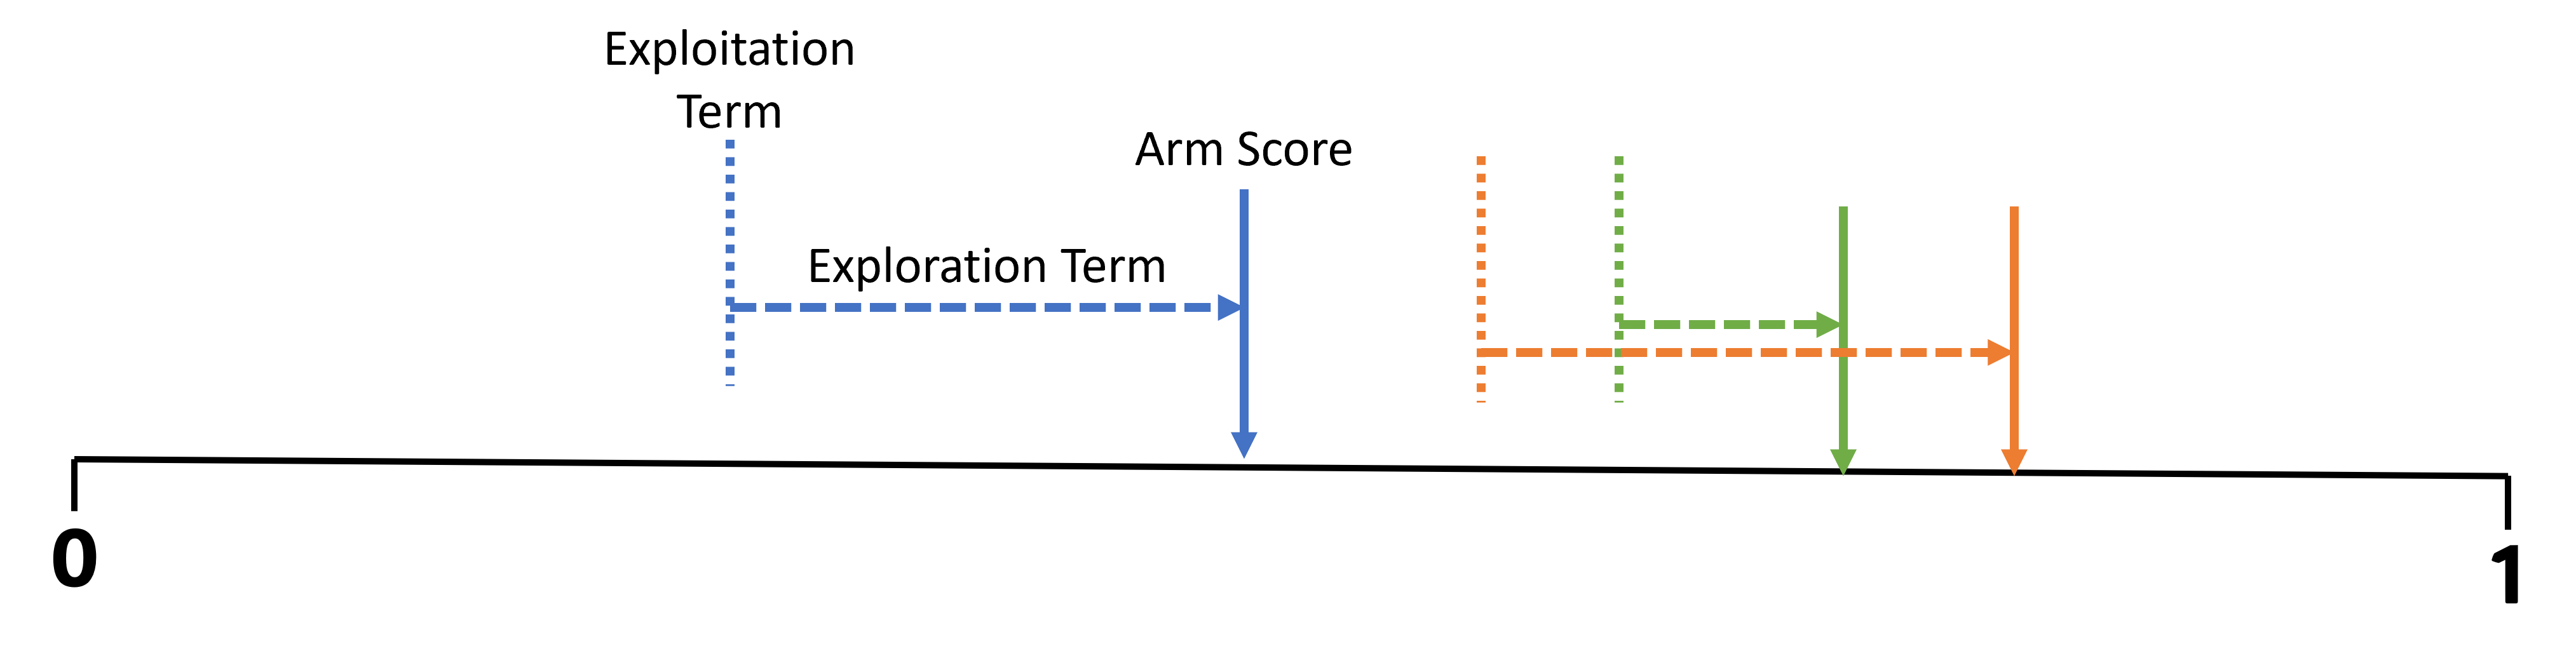
\includegraphics[width=1\textwidth]{report/images/UCB Image.png}}
    \caption{A Visual Aid to the UCB Algorithm}
    \label{fig:ucb_image}
\end{figure}



In general terms, any UCB algorithm can be described by:

$$
A_t = \arg\max_i \left[ \text{exploitation term} + \text{exploration term} \right]
$$

where the exploration term usually tends to zero as $t \rightarrow \infty$. For example, in the above figure \ref{fig:ucb_image}, the exploitation term is an indication of how "good" the arm is, whereas the exploration term is usually a measure of how unsure we are of the arm. Even though the \contour{green}{green} arm has a higher exploitation score, the \contour{orange}{orange} arm has more uncertainty around it, hence it's exploration score is higher 

More specifically in this project, we will use the UCB1 algorithm \cite{Slivkins_2019}, which uses this formula:

$$
A_t = \arg\max_i \left( Q_i +  \sqrt{\frac{c\log(t)}{N_i}} \right)
$$

For some confidence value $c$. We use $c = 2$ for optimal regret. This allows us to derive the sensible confidence bounds, since it gives a probabilistic guarantee of how likely our sample mean is to deviate from the true mean of an arm distribution.

For UCB, finite sample concentration inequality-based (FSCI) confidence intervals are preferred over Central Limit Theorem (CLT) confidence intervals due to their better performance when handling small sample sizes. CLT-based intervals rely on the assumption of having a large sample size (which ensures the sample mean converges to a normal distribution). However, in MAB problems, we sometimes have very limited data for some/all arms.

In contrast, FSCI-based confidence intervals such as Hoeffding's inequality, give bounds on the deviation of the sample mean from the true mean with high probability, even with very small sample sizes. This helps account for the inherent randomness of MAB, and the exploration-exploitation trade-off, as arms that have a poor sample mean calculated from very few attempts still have a good-enough guess for their true mean.

The algorithm can be summarized as follows:

\pseudobox{%
    \KwIn{List of arms $\armsList$ with unknown distributions $\armDistributionVect$, confidence value $c$, number of timesteps $\timeHorizon$}
    \KwOut{Selection strategy}
    \BlankLine
    \ForEach{arm $i = 1$ \KwTo $K$}{
        Initialise success rate $Q_i \leftarrow $\actionValueEstimate\newline
        Initialise count $N_i \leftarrow 0$
    }
    \BlankLine
    \For{$t = 1,\ldots, \timeHorizon$}{
        Choose arm $A_t \leftarrow \arg\max_i \left( Q_i + \sqrt{\frac{c\log(t)}{N_i}} \right)$\;
        Receive the reward $R_t$ by pulling arm $A_t$\;
        Increment count: $N_{A_t} \leftarrow N_{A_t} + 1$\;
        Update success rate: $Q_{A_t} \leftarrow \frac{S_{A_t}}{N_{A_t}}$
    }
}{Upper Confidence Bound (UCB) Algorithm}

In the UCB algorithm, it aims to balance the exploitation of arms with high estimated success rates and the exploration of arms with high uncertainty or limited exploration history:

\begin{itemize}
    \item $Q_i$ chooses greedily which arm to pick given their past success rates
    \item $\sqrt{\frac{c\log(t)}{N_i}}$ attempts to sway the greedy exploration, by adding some uncertainty to the result.
    \begin{itemize}
        \item If an arm hasn't been pulled very often, the uncertainty is very large, and vice versa. Therefore, over time, the algorithm becomes more and more `confident' about it's estimates.
        \item Due to the logarithmic nature of this particular uncertainty term, it'll slowly increase when arms aren't selected, but quickly shrink when they are. Therefore, the algorithm will tend to not `give up' on arms that appear to be sub-optimal, and will pull them infrequently until a significant score is obtained by another arm.
    \end{itemize}
\end{itemize}

One of the key advantages of UCB is that it naturally adapts its exploration strategy over time. As the algorithm collects more data and gains confidence in the success rates of different arms, the exploration bonus diminishes, leading to a more exploitation-focused strategy. In comparison to the previous algorithms, UCB offers a more systematic approach to exploration by considering uncertainty explicitly. Depending on the problem at hand, UCB can provide a more efficient trade-off between exploration and exploitation, potentially leading to better overall performance in various applications.

The regret bound for the UCB $\policy$ is sub-linear. Indeed, the rate is $O(\sqrt{n})$.

Finally, given a failure probability $\delta \in (0,1)$, we let $\ucb{a}{t}{\delta}$ denote the upper confidence bound on $\armPopulationMean{a}$ based on the first $t$ rounds,


\begin{theorem}[UCB regret bound]\label{thm:ucbRegretBound}
Suppose we have a stochastic bandit problem with time horizon $\timeHorizon \in \N$ and $\numArms \in \N$ with corresponding gaps $(\gap{i})_{i \in [\numArms]}$. Then letting $\ucbPolicy$ be the UCB policy with parameters $\delta$, $\totalFunction{a}{t}$ and $\empiricalMeanReward{a}{t}$, we have the following regret bound,
\begin{align*}
\cumulativeRegret{T}{\ucbPolicy} \leq 8 \sqrt{\timeHorizon \numArms \log(\timeHorizon)} + 3 \sum_{i=1}^{\numArms} \gap{i}.
\end{align*}
\end{theorem}

We shall now give a high-level description of the proof from this paper \cite{Lattimore_Szepesv´ar}. Recall that $\totalFunction{i}{\timeHorizon}$ denotes the number of times arm $i \in [\numArms]$ has been played over the time horizon $\timeHorizon$. We break down the regret for the UCB policy,

\begin{align}\cumulativeRegret{T}{\ucbPolicy} \leq \sum_{i=1}^{\numArms} \gap{i} \cdot \Ex(\totalFunction{i}{\timeHorizon}). \label{eq:ucb-breakdown}
\end{align}

Using the Law of Total Expectation, we can split up the $\Ex(\totalFunction{i}{t})$ by using a ``good event'' $G_i$, which is when:

\begin{enumerate}
    \item The best arm's mean is never underestimated
    \item The other's arm's upper bounds are never higher than the best arm's mean
\end{enumerate}

If we let $u_i$ \space be some number of observations st. the upper bound for sub-optimal arms don't exceed the best arm's mean, we get:

$$\Ex(\totalFunction{i}{t}) = \Ex(\mathbb{I}(G_i)\totalFunction{i}{t}) + \Ex(\mathbb{I}(G_i^c)\totalFunction{i}{t}) \leq u_i + \Prob(G_i^c) \cdot n.$$

We apply Hoeffding's inequality \ref{sec:hoeffding} obtain the bound,
$$\Prob(G_i^c) \leq n \delta + \exp\left(-\frac{ \gap{i}^2}{4} \left\lceil \frac{8\log(1/\delta)}{\gap{i}^2} \right\rceil\right)\leq (n+1)\delta.$$

Solving for $u_i$ from the definition, we get $u_i = \lceil \frac{2log(1/\delta)}{(1-c)^2\gap[i]^2} \rceil$. After setting $\delta = 1/n^2$, this leads to:

$$\Ex(\totalFunction{i}{t}) \leq 3 + \frac{16\log(t)}{\gap{i}^2}$$

So, we have for $\epsilon \in [0,1]$,
\begin{align*}
\cumulativeRegret{T}{\ucbPolicy} &\leq \sum_{i=1}^{\numArms} \gap{i} \cdot \Ex(\totalFunction{i}{\timeHorizon})
\\&= \sumindless \gap{i} \cdot \Ex(\totalFunction{i}{\timeHorizon})
+ \sumindgreater \gap{i} \cdot \Ex(\totalFunction{i}{\timeHorizon})
\\&= \timeHorizon \epsilon + \sum_{i=1}^{\numArms}\one_{\{\Delta_i \geq \epsilon\}}\left(3 \gap{i}+\frac{16 \log \timeHorizon}{\Delta_i}\right).
\end{align*}

If we set $\epsilon = \sqrt{16k \log \timeHorizon/\timeHorizon}$ we obtain 

$$R_\stoppingTime(\policy) \leq 8 \sqrt{\stoppingTime \numArms \log(\stoppingTime)} + 3 \sum_{i=1}^{\numArms} \gap{i}. \qed$$

Note we can make this bound gap-independent, by noticing $\gap{i} < 1 \forall i$, so we get:

$$R_\stoppingTime(\policy) \leq 8 \sqrt{\stoppingTime \numArms \log(\stoppingTime)} + 3.$$


\subsubsection{(Bernoulli) Thompson Sampling}
\label{sec:BernoulliThompsonSampling}
Thompson Sampling is another popular approach to MAB - unlike the Upper Confidence Bound (UCB) algorithm, Thompson Sampling approaches the problem from a Bayesian perspective, leveraging posterior probability distributions to make decisions about which arms to pull.

At its core, Thompson Sampling maintains a probabilistic model of the true success rate distribution for each arm. Instead of trying to estimate a single success rate for each arm with a single value, Thompson Sampling maintains an entire posterior distribution of success rates, which is updated as the algorithm collects more data.

The algorithm is named after William R. Thompson, who introduced it in his paper ``On the Likelihood that One Unknown Probability Exceeds Another in View of the Evidence of Two Samples'' \cite{Thompson_1933} in 1933. The central idea behind Thompson Sampling is to select arms for exploration and exploitation according to their sampled success rates from their respective distributions.

The Thompson Sampling algorithm can be summarized as follows:

\pseudobox{%
    \KwIn{List of arms $\armsList$ with unknown distributions $\armDistributionVect$, number of timesteps $\timeHorizon$}
    \KwOut{Selection strategy}
    \BlankLine
    \For{$t = 1,\ldots, \timeHorizon$}{
        Sample a success rate $\theta_i$ from the distribution $\armDistribution{i}$ associated with arm $i$ for all $i \in \numArms$\;
        Choose arm $A_t \leftarrow \arg\max_i \theta_i$\;
        Receive the reward $R_t$ by pulling arm $A_t$\;
        Update the distribution parameters for arm $A_t$ based on the observed reward;
    }
}{Thompson Sampling Algorithm}

Since we are discussing the Bernoulli bandit, the appropriate algorithm is the Bernoulli Thompson Sampling, often abbreviated to BernTS, which is outlined below. It uses the Beta distribution, which is very suitable for modeling probabilities in Bernoulli trials.

Importantly, this utilizes a "conjugate prior", which describes a prior distribution that, when combined with the likely-hood function, gives a posterior distribution in the same family as the prior. Specifically in the case, the Beta distributions acts as the Bernoulli's conjugate prior:

$$Beta(\alpha,\beta) \times Bernoulli(p) \propto Beta(\alpha',\beta')$$

This property greatly simplifies the process of updating beliefs based on incoming evidence, as it's much easier to calculate compared to e.g Dirichlet (used for vector uncertainty), where $Dirichlet(\alpha_1,\alpha_2) \times Bionomial \not\propto Dirichlet(\alpha_1',\alpha_2')$

Additionally, each arm $i \in [0, \numArms]$ is associated with a Beta distribution:

$$\armDistribution{i} \sim \mathrm{Beta}(S_i + \alpha_i, F_i + \beta_i)$$

In this algorithm, priors are introduced - any initial beliefs, or assumptions about the environment before any data is collected. $\alpha$ represents past "positive" experience, and conversely $\alpha$ represents past "negative" experience. By incorporating priors into BernTS, the algorithm starts with a base understanding of each arm's probabilities, which is refined over time, slowly becoming less influential as arms are explored, aiding the exploration/exploitation trade-off.

\pseudobox{%
    \KwIn{List of arms $\armsList$ with Bernoulli success probabilities $\theta_i$, number of timesteps $\timeHorizon$, priors $\alpha_i, \beta_i$}
    \KwOut{Selection strategy}
    \BlankLine
    \ForEach{arm $i = 1$ \KwTo $K$}{
        Initialise number of successes $S_i \leftarrow 0$\;
        Initialise number of failures $F_i \leftarrow 0$\;
    }
    \For{$t = 1,\ldots, \timeHorizon$}{
        Sample a success probability $\theta_i$ from $\text{Beta}(S_i + \alpha_i, F_i + \beta_i)$ associated with arm $i$ for all $i \in \numArms$\;
        Choose arm $A_t \leftarrow \arg\max_i \theta_i$\;
        Receive the reward $R_t$ by pulling arm $A_t$\;
        \If{$R_t = 1$}{
            $S_i \mathrel{+}= 1$
        }
        \Else{
            $F_i \mathrel{+}= 1$
        }
    }
}{Bernoulli Thompson Sampling Algorithm}


Thompson Sampling finds a balance between exploration and exploitation, since it has a built-in exploration mechanism, occasionally sampling arms that may not be currently considered the best arm based on existing data. Over time, the algorithm's estimates improve as more data is collected, leading to more accurate decisions.

Thompson Sampling's key advantages are its simplicity and adaptability. It naturally handles uncertainty and adjusts its exploration strategy based on observed data. This adaptability makes it particularly effective when arm success rate distributions may change over time.

However, the algorithm struggles to manage the computational complexity of sampling from complex distributions, especially when dealing with a large number of arms. Also, like other bandit algorithms, Thompson Sampling's performance can be affected by the choice of hyper-parameters (priors). Incorrect choices here can cause the algorithm to produce very unreliable results.\ref{sensitive_priors}


\subsubsection{Ripple Sampling}
\label{sec:ripple}

After exploring all of the above algorithms, I decided to design my own classical bandit algorithm - Ripple. It draws inspiration from established concepts like the UCB, Thompson sampling, and Greedy approaches. From UCB, it adopts the idea of deterministically choosing arms based on confidence bounds. This ensures that decisions are made with a certain level of certainty, maximizing the likelihood of selecting the most promising option. Additionally, Ripple incorporates elements of Thompson sampling by maintaining posterior distributions over the mean of each arm. Moreover, it embraces the Greedy strategy by selecting arms optimistically in each iteration, aiming to maximize potential gains.

The basic idea is that, at each time-step, it picks the arm that's most likely to have reasonable probability of having a high probability of success. This equates to:

$$A_t = \arg\max_{i \in [K]} \sup_{X_i \in \mathbb{R}} \left\{ X_i \suchthat \left| \Pr(\text{Arm } i \text{ has } \textbf{normalised} \text{ mean } X_i) - \rho \right| < \epsilon \right\}
$$

The two values we have to define are $\rho$ the \textbf{pessimism tolerance} and $\epsilon$ the \textbf{numerical tolerance}. $\rho$ is the probability that we count as reasonable for a potential probability $X_i$, and is chosen somewhat arbitrarily, usually around 0.01. $\epsilon$ is the tolerance between $X_i$ and $\rho$ to determine if they are close enough, and is typically a really small value such as $10^{-6}$.

We also must define a \textbf{normalised mean} - this is the probability that, given the empirical data up time $t$, that the arm has mean $X_i$, scaled across all possible means. When the probability of means is calculated using binomial distributions, we can say:

Let $S_i(t) := \sum_{i=1}^{t} \mathbb{I}(\action{i} = a)\cdot \reward{t-1}{a}$ to be the number of successes for arm i at time t. Then, we can let $x = X_i$, $s = S_i(t)$ and $m = \totalFunction{i}{t}$ for neatness, so we have:

\setlength{\jot}{10pt}
\begin{align*}
\bar{\Prob}(x) &= \frac{\Prob(x)}{\Prob(\frac{s}{m})} \\
&= \frac{\binom{m}{s}x^s (1-x)^{m-s}}{\binom{m}{s}\left(\frac{s}{m}\right)^s \left(1-\frac{s}{m}\right)^{m-s}} \\
&= \frac{x^s (1-x)^{m-s}}{\left(\frac{s}{m}\right)^s \left(1-\frac{s}{m}\right)^{m-s}}
\end{align*}
\setlength{\jot}{8pt}

We can see through both figures below that this outperforms both UCB and BernTS in both scenarios

\begin{figure}[h!]
    \centering
    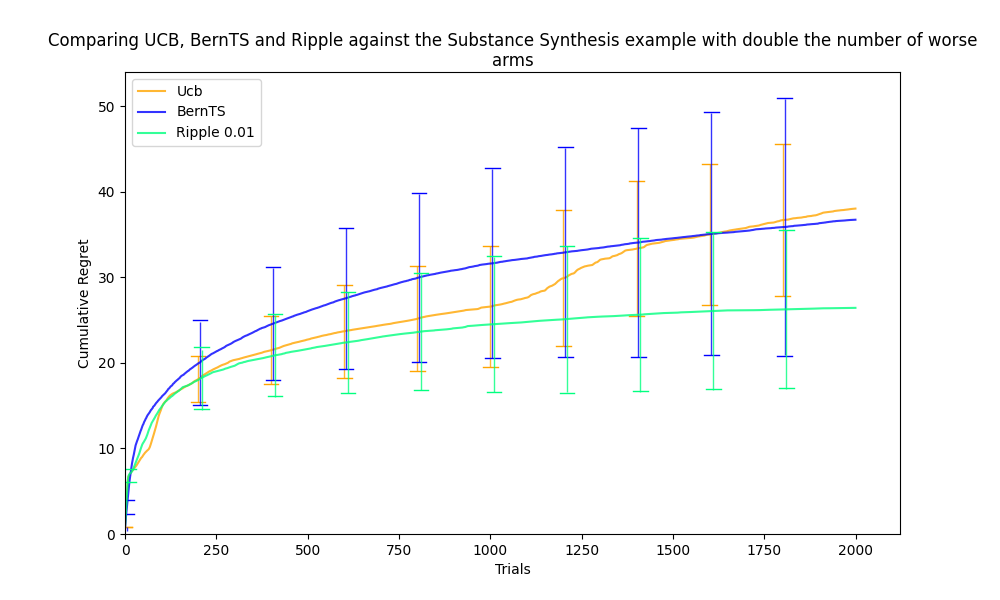
\includegraphics[width=17cm]{report/images/Ripple-Outperforms-BernTS-SS-Modified.png}
    \caption{Ripple's upper and lower bounds are both better than UCB and BernTS (showing double the time horizon)}
    \label{fig:ripple-cp}
\end{figure}

\begin{figure}[h!]
    \centering
    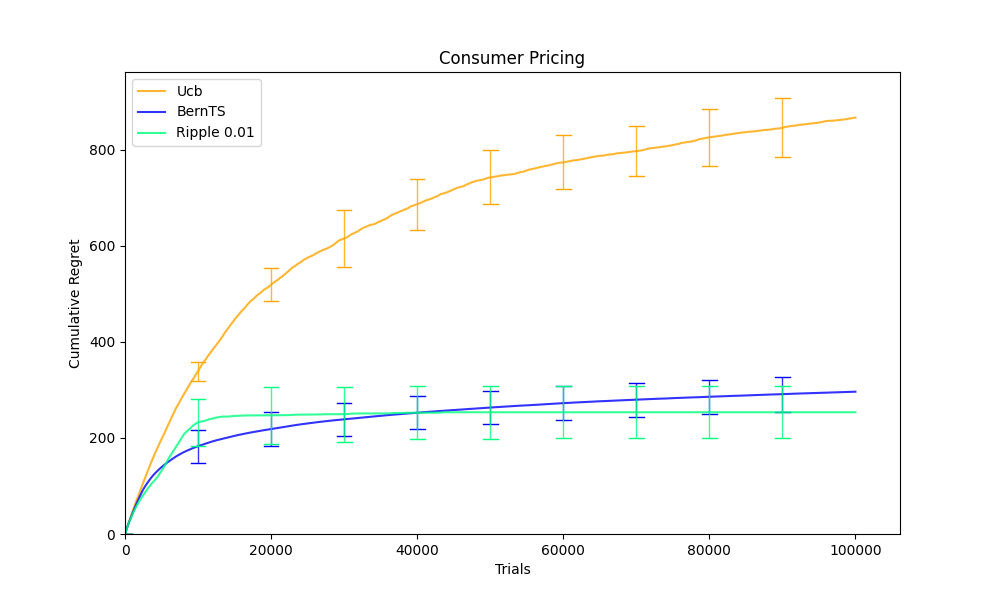
\includegraphics[width=17cm]{report/images/Ripple-Outperforms-BernTS-CP.png}
    \caption{Although Ripple starts off with more cumlative regret, past $\sim$10,000 trials it doesn't accumulate significant regret at all}
    \label{fig:ripple-cp}
\end{figure}

The algorithm can be summarized as follows:

\pseudobox{%
    \KwIn{List of arms $\armsList$ with unknown distributions $\armDistributionVect$, pessimism tolerance $\rho$, numerical tolerance $\epsilon$, number of timesteps $\timeHorizon$}
    \KwOut{Selection strategy}
    \BlankLine
    \ForEach{arm $i = 1$ \KwTo $K$}{
        Initialise success count $S_i \leftarrow 0$\newline
        Initialise number of plays $M_i \leftarrow 0$
    }

    \BlankLine
    \SetKwFunction{normProb}{normProb}
    \SetKwProg{Fn}{Function}{:}{}
    \Fn{\normProb{$x, s, m$}}{
        $a \leftarrow \frac{s}{m}$\;
        \Return $\frac{x^{s} (1-x)^{m-s}}{a^{s}  (1-a)^{m-s}}$\;
    }
    
    \BlankLine
    \For{$t = 1,\ldots, \timeHorizon$}{
        \For{$i \in [K]$}{
            Use binary search to find $X_i$ so $|\mathrm{normProb}(X_i, S_i, M_i) - \rho| \leq \epsilon$\;
            }
        Choose arm $A_t \leftarrow \arg\max_i X_i$\;
        Receive the reward $R_t$ by pulling arm $A_t$\;
        $M_i = M_i + 1$\;
        \If{$R_t = 1$}{
            $S_i \leftarrow S_i + 1$\;
        }
    }
}{Ripple Algorithm}

\chapter{Pure Exploration}
\label{cha:pureexploration}

\section{The Premise}
\label{sec:premise}
Moving on from our discussion of exploration-exploitation algorithms in MAB problems, we'll now explore the concept of pure exploration. Unlike exploration-exploitation, which has to balance between exploiting the best arm whilst exploring for better ones, pure exploration simplifies this by focusing solely on exploration. This means it doesn't care about being penalized choosing sub-optimal arms, as it's goal is to find the best arm as fast as possible with some certainty value.

Since in pure exploration we no longer care about cumulative regret, we have to redefine our performance measure. One popular method is using simple regret, which is defined as "the expected regret to be chosen after time t by policy $\policy$":

$$\simpleRegret{t, \policy}{\policy} = \Ex_{\policy}(\gap{A_{t+1}}).$$

Intuitively, relating to our Ice Cream example \ref{ex:ice-cream}, this represents the expected performance difference between the best ice cream and the selected one. Naturally, we want this to be as small as possible, to minimize the probability we choose a worse ice cream, although we are constrained by two factors:

\begin{itemize}
    \item How long we have (t)
    \item How certain we want to be we've got the best arm ($\rho$)
\end{itemize}

\section{Algorithms for pure exploration - uniform}
\label{sec:simpleregret}

Uniform exploration is the simplest form of algorithm for pure exploration scenarios. Similarly to the Greedy algorithm \ref{sec:Greedy}, it samples arms in such a way that the outcome is a uniform selection. However for the Uniform exploration policy, we ensure each arm is selected perfectly uniformly. This means we have no notion of an action value estimate:

\pseudobox{%
    \KwIn{List of arms $\armsList$ with unknown distributions $\armDistributionVect$}
    \KwOut{Selection strategy, best arm}
    \BlankLine
    \ForEach{arm $i = 1$ \KwTo $K$}{
        Initialise number of successes $S_i \leftarrow 0$
    }
    \BlankLine
    \For{$t = 1,2,\ldots$}{
        Choose arm $A_t = t \mod{K}$\newline
        Receive the reward $R_t$ by pulling arm $a$;\newline
        Increment successes: $S_a \leftarrow S_a + R_t$\newline
     }
    return arm $A_i$ with the highest number of successes: $A_i \leftarrow \arg\max_i S_a$ \newline

}{Uniform Algorithm}

\section{Fixed Confidence}
\label{sec:fixedconfidence}

In the previous chapter, we had some notion of certainty of our decisions, such as UCB \ref{sec:UCB} and Ripple \ref{sec:ripple}. However, our understanding was obfuscated by the exploration and exploitation factors. An exception to this is when $t \rightarrow \infty$, but this is unrealistic, and doesn't align with real-world situations, as demonstrated by the Substance Synthesis example \ref{ex:substance-synthesis}.

However, in pure exploration, our only "drive" is exploration, which makes defining a failure probability parameter $\failureProb$ much easier. Hence, an algorithm's goal is to find the best arm, with $(1-\failureProb)$ certainty, with as few samples as possible i.e before some stopping time $\stoppingTime$. Naturally, the exact value of $\failureProb$ will vary depending on the scenario - for our Substance Synthesis example \ref{ex:substance-synthesis}, we may have our $\failureProb$ relatively high, if we expect there to be a very large difference in the results of each resistor. However, in the later stages, when changes are comparatively much smaller, we may choose a very small value for $\failureProb$ so that we're very certain which changes have made an improvement. In order to compare any strategies, let us define:

\begin{definition}\label{def:method}
    The triple $(\policy, \stoppingTime, \selectionRule)$ is a \textbf{method} $\method$, given a policy $\policy$, stopping time $\stoppingTime$, and selection rule $\selectionRule$.
\end{definition}

\ognote{Elaborate on specifics of policy, stopping time and selection rule}

\begin{definition}\label{def:soundess}
A method  $\method = (\policy, \stoppingTime, \selectionRule)$ is said to be \textbf{sound} with failure probability $\failureProb$ if for all  $v \in \banditSpace$,

$$\Prob_{}(\stoppingTime < \infty  \text{ and }  \gap{\selectionRule}(v) > 0) \leq \failureProb.$$

Equivalently:

$$\Prob_{}(\stoppingTime < \infty  \text{ and }  \gap{\selectionRule}(v) = 0) \geq 1-\failureProb.$$

\end{definition}

In other words, a triple is sound if, which probability of failure $\failureProb$: The policy stops, and the current gap is optimal. The $\stoppingTime < \infty$ is needed, since a triple that doesn't stop is meaningless.

Naturally, we desire some method that has policy $\policy$ that minimizes the stopping time $\stoppingTime$ and failure probability $\failureProb$. However, similar to exploration-exploitation bandits, we must strike some balance between efficiency and certainty - increasing the stopping time of $\stoppingTime$ decreases the confidence $\failureProb$ that the chosen arm is optimal. Conversely, letting the confidence $\failureProb$ increase slightly can decrease the stopping time from $\stoppingTime$ a large amount.


\section{Track-and-Stop Strategies}
\label{sec:trackandstop}
% Explain Section 33.2.2 and try to make sense of Algorithm 21 and Theorem 33.6.
It has been shown previously that the expected stopping time $\stoppingTime$ for a MAB with fixed confidence $\failureProb$ is bounded by below as follows:

\begin{theorem}
For a MAB with arm distributions $\armDistributionVect$, some method $\method = (\policy, \stoppingTime, \selectionRule)$, and failure probability $\failureProb$, $\forall v \in \banditSpace:$ \ognote{Theorem 33.5 in Lattimore}

$$\Ex(\stoppingTime) \geq c^*(v) \times log\left({\frac{1}{4(1-\failureProb)}}\right)$$

$$for \quad \ognote{Unsure}$$
\end{theorem}

\ognote{Insert lower bound statement}

Sadly, we cannot construct an algorithm that outperforms this \ognote{the lower bound}; however, we can create one that ensures all potential outcomes are as close to the lower bound as possible. In order to do this, such an algorithm would have to estimate each arm's underlying mean $\armPopulationMean{a}$ by sampling in proportion to the empirical mean $\empiricalMeanReward{a}{t}$ for $t \leq \stoppingTime$.

However, this can lead to some arms being "starved" if we initially get unfortunately poor results from the first few samplings, similarly to greedy strategies mentioned previously\ref{sec:Greedy}. Hence, we must impose some "resource equity" by requiring us to sample each arm at least some number of times at each time measure, which hopefully ensures $\empiricalMeanReward{a}{t}$ is close to $\armPopulationMean{a}$ for sufficiently large $t$


Part of what makes pure exploration algorithms interesting is that they can terminate early whilst not having a narrow uncertainty around each arm's true mean $\armPopulationMean{a}$. This is because they typically hold estimates of each arm's true distribution $\armDistribution{a}$, which is updated at each time step. The uncertainty can then be calculated w.r.t these estimated distributions 

The high-level intuition of the Track-and-Stop algorithm is as follows:

\begin{itemize}
    \item While there is a reasonable probability multiple arms could be optimal:
    \begin{itemize}
        \item If the arm that has been selected least often hasn't been selected at least $\sqrt{t}$ times:
        \begin{itemize}
            \item Choose this arm
        \end{itemize}
        \item Otherwise:
        \begin{itemize}
            \item Choose arm i that maximizes (t * average) - no. times selected
        \end{itemize}
    \end{itemize}
    \item Set the selection rule to the arm with the highest mean at this time-step, and set the stopping time
\end{itemize}

The pseudo-code for the Track-and-Stop algorithm is defined as follows:

\pseudobox{%
    \KwIn{Confidence $\failureProb$, $\beta_t(\failureProb)$}
    \KwOut{Selection strategy}
    \BlankLine
    t = 0\newline
    \ForEach{arm $i = 1$ \KwTo $K$}{
        Choose arm $A_{t+1} \leftarrow i$
    }
    \BlankLine
    \While{$Z_t < \beta_t(\failureProb)$}{
        \If{$\arg\min_{i \in [K]}T_i(t) \leq \sqrt{t}$}{
            Choose arm $A_{t+1} \leftarrow \arg\min_{i \in [K]} T_i(t)$;
        }
        \Else{
            Choose arm $A_{t+1} \leftarrow \arg\max_{i \in [K]} (t * \empiricalMeanReward{a}{t} - T_i(t))$;
        }
     }
    return selection rule $\selectionRule = i^*(\hat{v}(t))$, stopping time $\stoppingTime = t$\newline

}{Track-And-Stop Algorithm}

\newcommand{\defineZedTee}[1]{\frac{1}{2}\inf\limits_{\aDifBandit \in \banditSpace_{alt}(\vectorBanditMeans(#1))}
\sum_{i=1}^k T_i(#1) \left( \vectorBanditMeans_i(#1) - \aDifBandit_i(#1) \right)^2}

\url{https://docs.scipy.org/doc/scipy/tutorial/optimize.html}

We define $Z_t = \defineZedTee{t}$ and $\beta_t(\failureProb)$ to be some function that determines stopping time

We now have to show the Track-And-Stop algorithm is sound\ref{def:soundess} with $\failureProb$, given some stopping time $\stoppingTime = \beta_t(\failureProb)$, which we do as follows:

% We firstly need to assume \maxMeanArm

\ognote{Complete rubbish - needs rewriting}
arbitrarily arm $i=1$ is best, in that $\armDistribution{1} = \maxArmDistribution$. This naturally means we want the best arm to be picked constantly after the stopping time, so $\maxMeanArm{t} = 1$ for $\stoppingTime + 1 \leq t < \infty$, since we must account for that the algorithm stops at time $\stoppingTime$, then queries afterwards
\ognote{Complete rubbish - needs rewriting}

Now, we note that:
\begin{align*}
&\mathrel{\phantom{=}}\left\{\textbf{bandits which disagree with the empirical distribution over what the best arm is} \right\} \\
&\mathrel{\phantom{=}}\subseteq \left\{\textbf{bandits where the algorithm stops at our stopping time}\right\}
\end{align*}

Which leads to:
$$\left\{ v \in \banditSpace_{alt}(\maxMeanArm{{\stoppingTime}}) \right\} \subseteq \left\{ Z_{\stoppingTime} < \beta_{\stoppingTime}(\failureProb)\right\}$$

$$\left\{ 1 \notin \maxMeanArm{{\stoppingTime}} \right\} = \left\{ v \in \banditSpace_{alt}(\maxMeanArm{{\stoppingTime}}) \right\} \subseteq \left\{ \defineZedTee{\stoppingTime} < \beta_{\stoppingTime}(\failureProb)\right\}$$

So our target equation is the following:

\label{tar:track-and-stop}
$$\Prob( 1 \notin \maxMeanArm{{\stoppingTime}}) \leq \Prob\left( \defineZedTee{\stoppingTime} \geq \beta_{\stoppingTime}(\failureProb)\right) \leq \failureProb$$

\seperator

Let us define:

$$S_{i_s} := \frac{s}{2}(\vectorBanditMeans_{i}(\stoppingTime^{-1}(s)) - \armPopulationMean{i})^2 \textbf{ where } \stoppingTime^{-1}(s) := min \{ t \in \naturals : \stoppingTime_{i}(t) = s \}$$

By Lemma\ref{lem:upperBoundSeq}:
$$\implies \Prob(\exists s \in \naturals : S_{i_s} \geq \log{s(s+1)} + \log{\frac{1}{\failureProb}}) \leq \failureProb$$

If we let $g(s) = \log{\failureProb(\failureProb + 1)}$, we meed the conditions of Lemma\ref{lem:increasingSeqUpper}, so:

$$\implies \Prob \left(\exists (s_i)_{i=1}^{k} : \sum_{i=1}^{k}S_{i_s} \geq k ((\log{\sum_{i=1}}s_i)(\log{\sum_{i=1}}s_i + 1)) + x \right) \leq \left(\frac{x}{k}\right)^k e^{k-x}$$

$$\implies \Prob \left(\exists t \in \naturals : \frac{1}{2}\sum_{i=1}^{k}T_i(t)(\vectorBanditMeans_{i}(t) - \aDifBandit_{i}(t))^2 \geq k ((\log{t})(\log{t + 1})) + x \right) \leq \left(\frac{x}{k}\right)^k e^{k-x}$$

We know that if $t \in \naturals$ exists, then the statement must also hold for $\stoppingTime \geq t$:

$$\implies \Prob \left(\frac{1}{2}\sum_{i=1}^{k} T_i(\stoppingTime)(\vectorBanditMeans_{i}(\stoppingTime) - \aDifBandit_{i}(\stoppingTime))^2 \geq k ((\log{\stoppingTime})(\log{\stoppingTime + 1})) + x \right) \leq \left(\frac{x}{k}\right)^k e^{k-x}$$

Now, we get to the point where we must define $\beta_{t}(s)$. If we say $\beta_{t}(s) := k * log\left(t(t+1)\right) + \failureProb^{-1}(\failureProb)$ with $\failureProb(s) := \left(\frac{x}{k}\right)^k e^{k-s}$, then we have $\failureProb^{-1}(\failureProb) = x$ and $\failureProb(x) = \failureProb$, so:

$$\implies \Prob \left(\frac{1}{2}\sum_{i=1}^{k} T_i(\stoppingTime)(\vectorBanditMeans_{i}(\stoppingTime) - \aDifBandit_{i}(\stoppingTime))^2 \geq \beta_{\stoppingTime}(s) \right) \leq \left(\frac{x}{k}\right)^k e^{k-x}$$

$$\implies \Prob \left(\frac{1}{2}\inf\limits_{\aDifBandit \in \banditSpace_{alt}(\vectorBanditMeans(\stoppingTime))}\sum_{i=1}^{k} T_i(\stoppingTime)(\vectorBanditMeans_{i}(\stoppingTime) - \aDifBandit_{i}(\stoppingTime))^2 \geq \beta_{\stoppingTime}(s) \right) \leq \left(\frac{x}{k}\right)^k e^{k-x}$$

We have now met the target\ref{tar:track-and-stop} equation, so we have:

$$\beta_{t}(s) = k * log\left(t(t+1)\right) + x$$
$$Z_{t}(\vectorBanditMeans) = \frac{1}{2}\inf\limits_{\aDifBandit \in \banditSpace_{alt}(\vectorBanditMeans)}\left(\sum_{i=1}^{k} T_i(t)(\vectorBanditMeans_{i}(t) - \aDifBandit_{i})^2\right)$$
$$\epsilon = \left(\frac{x}{k}\right)^k e^{k-x}$$

Perhaps the simplest way will be to use the expression in [33.4a in Lattimore book] and re-parameterise $\alpha$ as a vector $\beta_1,...,\beta_K \in \R $ via $ \alpha_i = e^{\beta_i}/(\sum_j e^{\beta_j})$. This way you don't need any additional constraints to encode probability vectors.

Let $\alpha_i = \frac{e^{\beta_i}}{c}$ with $c := \sum_j e^{\beta_j}$

Using that, and that $\sigma_i = 1 \forall i$:
$$\inf\limits_{\aDifBandit \in \banditSpace_{alt}(\vectorBanditMeans)}\left(\sum_{i=1}^{k} \alpha_i D(\vectorBanditMeans_{i}(t), \aDifBandit_{i})\right) = \frac{1}{2}\min_{i>1}\frac{\alpha_1 \alpha_i \gap{i}^2}{\alpha_1 \sigma_i^2 + \alpha_i \sigma_1^2} = \frac{1}{2}\min_{i>1}\frac{\gap{i}^2}{c} \frac{e^{\beta_1} e^{\beta_i}}{e^{\beta_1} + e^{\beta_i}}
$$

With $J(\beta):=\sum_{j=1}^K e^{\beta_j}$ we can define:
\[F(\beta):= \frac{1}{2}\min_{i>1}\frac{\alpha_1 \alpha_i \gap{i}^2}{\alpha_1 \sigma_i^2 + \alpha_i \sigma_1^2}=\frac{1}{2J(\beta)}\min_{i>1}   \frac{\Delta_i^2}{\sigma_i^2e^{-\beta_i} +\sigma_1^2 e^{-\beta_1} }\]

This is quite difficult to evaluate, since the minimisation may result in the values of $e^{-\beta_i}$ getting large enough such that the whole expression gets so small it \textquotedblleft rounds\textquotedblright\space down to zero, which isn't very helpful. Therefore, we can take to log and minimise over that

So we have:
\begin{align}
\log(F(\beta)) =\log\left(\min_{i>1}\frac{\alpha_1 \alpha_i \gap{i}^2}{\alpha_1 \sigma_i^2 + \alpha_i \sigma_1^2}\right)
=\log\left(\frac{1}{2J(\beta)}\min_{i>1}   \frac{\Delta_i^2}{\sigma_i^2e^{-\beta_i} +\sigma_1^2 e^{-\beta_1} }\right) \\
=\log\left(\frac{1}{2J(\beta)}\right) + \log\left(\min_{i>1} \frac{\Delta_i^2}{\sigma_i^2e^{-\beta_i} +\sigma_1^2 e^{-\beta_1} }\right) \\
=-\log\left(2\right) -\log\left(J(\beta)\right) + \min_{i>1} \log\left(\frac{\Delta_i^2}{\sigma_i^2e^{-\beta_i} +\sigma_1^2 e^{-\beta_1} }\right) \\
\log(F(\beta))=-\log\left(2\right) -\log\left(J(\beta)\right) + \min_{i>1} \left(2\log\left(\Delta_i\right) -\log\left({\sigma_i^2e^{-\beta_i} +\sigma_1^2 e^{-\beta_1} }\right)\right)
\end{align}

Note, when minimising this, the \textquotedblleft$-\log\left(2\right)$\textquotedblright\space makes no difference, so we can exclude it for those purposes. So, we have:

\begin{align}
Z_{t}(\vectorBanditMeans) = \frac{1}{2}F(\beta)
\implies Z_{t}(\vectorBanditMeans) = \frac{1}{2}e^{\log(F(\beta)) }
= \frac{1}{2}e^{-\log\left(2\right) -\log\left(J(\beta)\right) + \min_{i>1} \left(2\log\left(\Delta_i\right) -\log\left({\sigma_i^2e^{-\beta_i} +\sigma_1^2 e^{-\beta_1} }\right)\right)}
\end{align}

\lstset{language=Python, % set programming language basicstyle=\small\ttfamily, % basic font style stringstyle=\color{DarkGreen}, otherkeywords={0,1,2,3,4,5,6,7,8,9}, keywordstyle=\color{Blue}, % keyword style commentstyle=\ttfamily \color{DarkGreen}, numbers=left, % display line numbers on left numberstyle=\ttfamily\color{Gray}\footnotesize, % line numbers breaklines=true, breakatwhitespace=true, }

\newpage

\begin{lstlisting}[language=Python]
# Put the code 'ere
\end{lstlisting}
\chapter*{Simulations of classical and pure exploration}
\label{cha:simulations} % (labels for cross referencing)
\blindtext[1]
\chapter*{Conclusion}
\label{cha:conclusion} % (labels for cross referencing)

The aim of this project was to, firstly, understand and compare various different MAB algorithms, both in the traditional and pure exploration setting. Secondly, I wanted to implement these algorithms in code to learn strengths and weaknesses they have which are not obviously apparent when dealing with just the mathematical formulae.

The results demonstrate that there is no single algorithm for all MAB scenarios, as they each have specific strengths and weaknesses. The algorithms are either very adaptable, like Epsilon-Greedy and BernTS, or work better for tailored cases, such as UCB and Randomized.

I've shown that Epsilon-Greedy can be customized to fit the specific MAB scenario, however actually finding the correct \epsilonFunction \space to use is usually a case of trial-and-error, which is quite counterproductive, since it uses considerable resources in the process. BernTS can quite easily use prior data to decrease regret by a significant margin, however it can be overly sensitive to the priors selected, which can lead to unnecessary regret accumulation.

In contrast, I've shown that UCB works very well in it's own domain of bandits, specifically those with low numbers of arms and a low spread in the means. Unfortunately, there's no adaptability for different scenarios, other than changing how it calculates it's exploration and exploitation terms, which are an intrinsic part of this version of UCB. While virtually any other algorithm outperforms it, Randomized possesses one unique strength: its absolute lack of strategy ensures consistent, albeit consistently poor, outcomes.

In summary, this project shows the varied strengths and weaknesses of MAB algorithms, emphasizing the importance of tailored approaches. No one algorithm comes out as universally optimal, underscoring the need for careful consideration of specific MAB scenarios when selecting an algorithm.

\printbibliography[title={References}]

\appendix
% Theorems

\chapter{Appendix}\label{ch:appendix}

\section{Key tools from probability theory}

\label{sec:hoeffding}

\begin{theorem}[Hoeffding's Inequality]
Let $X_1, X_2, \ldots, X_n$ be independent random variables bounded in the interval $[a, b]$. Define the sample mean as $\bar{X}_n = \frac{1}{n}\sum_{i=1}^{n} X_i$. Then, for any $\epsilon > 0$, 
$$P\left(\left|\bar{X}_n - \mathbb{E}(\bar{X}_n)\right| \geq \epsilon\right) \leq 2 \exp\left(-\frac{2n\epsilon^2}{(b - a)^2}\right).$$
\end{theorem}

% Proofs
\section{Proofs of key results}

\subsection{Proof of \nameref{thm:ucbRegretBound}}
\label{app:proof_theorem_a}


\begin{proof}[Proof of Theorem \ref{thm:ucbRegretBound}]

We firstly assume, without loss of generality, that $\armPopulationMean{1} = \maxPopulationMean$. Then, we break down the regret as follows:

\begin{align*}
\cumulativeRegret{T}{\ucbPolicy} &\leq \sum_{i=1}^{\numArms} \gap{i} \cdot \Ex(\totalFunction{i}{t})
\end{align*}

The key idea now is to define a "good event" - ideally, we want:

\begin{enumerate}
    \item The best arm's mean to never be underestimated.
    \item The other arm's upper bound is never higher than the best arm's mean.
\end{enumerate}

Hence, we get:

\begin{align*}
G_i &= \left\{ \armPopulationMean{1} < \min_{i \in [\numArms]} UCB(i) \right\}
\cap \left\{ \armPopulationMean{i} + \sqrt{\frac{\log(t)}{\totalFunction{i}{t}}} < \mu_1 \right\}
\end{align*}

If $G_i$ occurs, then $\totalFunction{i}{t} \leq u_i$ for all arms, and if not, $\totalFunction{i}{t} \leq t$. We also assume $G_i^c$ is small. Hence, by the Law of Total Expectation:

\begin{align*}
\Ex(\totalFunction{i}{t}) &= \Ex(\mathbb{I}\{G_i\}\totalFunction{i}{t}) + \Ex(\mathbb{I}\{G_i^c\}\totalFunction{i}{t}) \leq u_i + \Prob(G_i^c) \cdot n
\end{align*}

Now, $\Prob(G_i^c)$ isn't very helpful at the moment, but:

\begin{align*}
G_i^c &= \left\{\armPopulationMean{1} \geq \min_{i \in [\numArms]} UCB(i)\right\}
\cup \left\{\armPopulationMean{i} + \sqrt{\frac{\log(t)}{\totalFunction{i}{t}}} \geq \mu_1 \right\}
\end{align*}

The first of these sets is decomposed using the definition of UCB:

\begin{align*}
\left\{ \mu_1 \geq \min_{i \in [\numArms]} UCB(i) \right\}
&\subset \left( \mu_1 \geq \min_{j \in [\numArms]} \hat{\mu}_j + \sqrt{\frac{2\log(1/\delta)}{j}} \right)\\
&= \bigcup_{j \in [\numArms]} \left( \mu_1 \geq \hat{\mu}_j + \sqrt{\frac{2\log(1/\delta)}{j}} \right) \quad \text{(Standard set theory)}
\end{align*}

Hence, we can generate a sum of independent subgaussian random variables:

\begin{align*}
\Prob(\mu_1 \geq \min_{i \in [\numArms]} UCB(i))
&\leq \Prob \left(\bigcup_{j \in [\numArms]} \left( \mu_1 \geq \hat{\mu}_j + \sqrt{\frac{2\log(1/\delta)}{j}} \right) \right) \\
&\leq \sum_{j=1}^{n} \Prob \left( \mu_1 \geq \hat{\mu}_j + \sqrt{2\log(1/\delta)} \right) \\
&\leq exp(-\frac{\numArms \times \sqrt{2\log(1/\delta)}^2}{2 \times 1^2}) \\
&\leq \numArms exp(-\frac{2\log(1/\delta)}{2}) \\
&\leq \numArms exp(-\log(1/\delta)) \\
&= \numArms \delta
\end{align*}

The second set we can bound relatively simply assuming we've chosen our $u_i$ large enough such that $\gap{i} - \sqrt{\frac{2\log(1/\delta)}{u_i}} \geq c \gap{i}$ for some c. Then:

\begin{align*}
\Prob\left( \hat{\mu}_i + \sqrt{\frac{\log(t)}{\totalFunction{i}{t}}} \geq \mu_1 \right)
&= \Prob\left( \hat{\mu}_i + \sqrt{\frac{\log(t)}{\totalFunction{i}{t}}} \geq \armPopulationMean{i} + \gap{i} \right) \quad \text{Since $\mu_1 = \armPopulationMean{i} + \gap{i}$} \\
&= \Prob\left( \hat{\mu}_i - \armPopulationMean{i} \geq \gap{i} - \sqrt{\frac{\log(t)}{\totalFunction{i}{t}}} \right) \\
&= \Prob\left( \hat{\mu}_i - \armPopulationMean{i} \geq c \gap{i} \right)
\leq exp(-\frac{u_i c^2 \gap{i}^2}{2})
\end{align*}

Hence, we now have

\begin{align*}
\Prob(G_i^c) &\leq n \delta + \exp\left(-\frac{u_i c^2 \gap{i}^2}{2}\right)
\end{align*}

Which leads back to:

\begin{align*}
\Ex(\totalFunction{i}{t}) &\leq u_i + n \left(n \delta + \exp\left(-\frac{u_i c^2 \gap{i}^2}{2}\right)\right)
\end{align*}

Now, choosing $u_i$ can be simple by rearranging the following:

\begin{align*}
& \gap{i} - \sqrt{\frac{2\log(1/\delta)}{u_i}} \geq c \gap{i} \\
& u_i \geq \frac{2\log(1/\delta)}{(1-c)^2\gap{i}^2} \\
& u_i = \lceil \frac{2\log(1/\delta)}{(1-c)^2\gap{i}^2} \rceil \quad \text{is a trivial solution.}
\end{align*}

Picking the natural choice  of $\delta = \frac{1}{t^2}$, this leads to:

\begin{align*}
\Ex(\totalFunction{i}{t}) &\leq u_i + t \left(t \delta + \exp\left(-\frac{u_i c^2 \gap{i}^2}{2}\right)\right) \\
&= u_i + t^2\delta + t\exp\left(-\frac{u_i c^2 \gap{i}^2}{2}\right) \\
&= \lceil \frac{2\log(1/\delta)}{(1-c)^2\gap{i}^2} \rceil + 1 + t^{1 - \frac{2c^2}{(1-c)^2}} \\
&= \lceil \frac{4\log(t)}{(1-c)^2\gap{i}^2} \rceil + 1 + t^{1 - \frac{2c^2}{(1-c)^2}}
\end{align*}

Now, we just need to find a suitable value for $c \in (0, 1)$. To minimize this expression:
\begin{itemize}
  \item The 1st term wants $c$ to be as small as possible.
  \item The 2nd term is a small constant, and can be ignored
  \item The 3rd term will be polynomial unless $\frac{2c^2}{(1-c)^2} \geq 1 \implies c \geq \sqrt{2}-1  \approx 0.414$.
\end{itemize}

In the proof by Lattimore and Szepesv´ar here\cite{Lattimore_Szepesv´ar}, they use c=1/2, which leads to:

\begin{align*}
\Ex(\totalFunction{i}{t}) &\leq \lceil \frac{4\log(t)}{(1-c)^2\gap{i}^2} \rceil + 1 + t^{1 - \frac{2c^2}{(1-c)^2}} \\
&= \lceil \frac{4\log(t)}{\frac{1}{4}\gap{i}^2} \rceil + 1 + t^{1 - \frac{1/2}{1/4}} \\
&= \lceil \frac{16\log(t)}{\gap{i}^2} \rceil + 1 + t^{-1} \\
&\leq \left( \frac{16\log(t)}{\gap{i}^2} + 1\right) + 1 + t^{-1} \\
&\leq 3 + \frac{16\log(t)}{\gap{i}^2} \quad \text{Since $t^{-1} \leq 1$}
\end{align*}

Which neatly resolves when plugged back into the original equation. By using decomposition, and supposing a mystery cutoff value $\lambda$, we have:

\begin{align*}
\cumulativeRegret{T}{\ucbPolicy} &\leq \sum_{i=1}^{\numArms} \gap{i} \cdot \Ex(\totalFunction{i}{t}) \\
&\leq \sum_{i: \gap{i} < \lambda}^{\numArms} \gap{i} \cdot \Ex(\totalFunction{i}{t}) + \sum_{i: \gap{i} \geq \lambda}^{\numArms} \gap{i} \cdot \Ex(\totalFunction{i}{t}) \\
&\leq n \lambda + \sum_{i: \gap{i} \geq \lambda}^{\numArms} \left( 3 + \frac{16\log(t)}{\gap{i}^2} \right)  \\
&\leq n \lambda + \frac{16k\log(t)}{\gap{i}^2} + 3 \sum_{i: \gap{i} \geq \lambda}^{\numArms} \gap{i} \\
\cumulativeRegret{T}{\ucbPolicy} &\leq 8 \sqrt{tk \log(t)} + 3 \sum_{i=1}^{\numArms} \gap{i} 
\end{align*}

Once we set $\lambda = \sqrt{\frac{16klog(n)}{n}}$.

\end{proof}


\label{lem:upperBoundSeq}
\begin{lemma}
Let $(X_t)_{t=1}^\infty$ be a sequence of independent Gaussian random variables with mean $\mu$ and unit variance. Let $\hat{\mu}_n = \frac{1}{n} \sum_{t=1}^n X_t$. Then, for any $\delta > 0$:
$$
\Prob\left(\exists n \in \mathbb{N}^+ \text{ st. } \frac{n}{2} (\hat{\mu}_n - \mu)^2 \geq \log\left(\frac{1}{\delta}\right) + \log(n(n + 1))\right) \leq \delta.
$$
\end{lemma}

\label{lem:increasingSeqUpper}
\begin{lemma}
Let $g : \mathbb{N} \to \mathbb{R}$ be increasing, and for each $i \in [k]$, let $S_{i_1}, S_{i_2}, \ldots$ be an infinite sequence of random variables such that for all $\delta \in (0, 1)$,
$$
P \left(\exists s \in \mathbb{N} : S_{is} \geq g(s) + \log\left(\frac{1}{\delta}\right)\right) \leq \delta.
$$
Then, provided that $(S_i)_{i=1}^k$ are independent and $x \geq 0$,
\[
P \left(\exists s \in \mathbb{N}^k : \sum_{i=1}^k S_{is_i} \geq kg \left(\sum_{i=1}^k s_i\right) + x\right) \leq \left(\frac{x}{k}\right)^k e^{k-x}.
\]
\end{lemma}


\end{document}
